\section{Design}
In order to measure enjoyability of landmark navigation in combination with game activities in a location-based game (LBG), we developed a LBG that takes place in Aalborg, Denmark and the area of three street art paintings \cite{streetart} that were used as points of interest (POIs). The game makes players walk between the three POIs on a route with a total length of 1.8km and a distance of 0.9km between POIs (see Figure \ref{FinalRoute}). Due to requirements from the method of the experiment as described in the Experiment section, the particular route was chosen on the basis of it having approximately the same amount of intersections in the road between POIs, as well as approximately the same distance between the POIs.

\begin{figure}[hbtp]
\centering
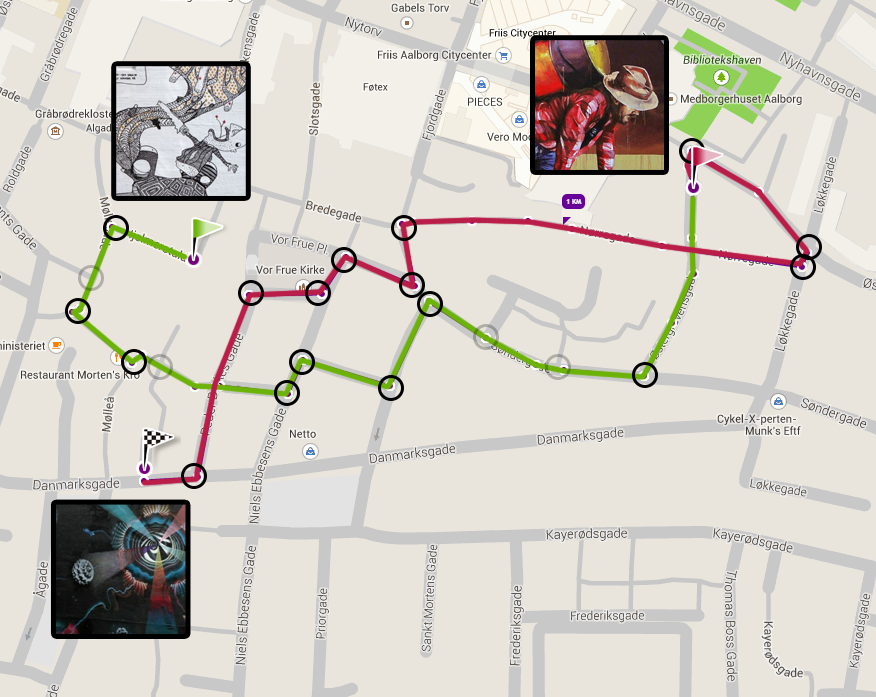
\includegraphics[scale=0.2]{Pics/FinalRoute.png}
\caption{The route between the three street art paintings.}
\label{FinalRoute}
\end{figure}

\subsection{Choice of Navigational Game Activity}
In the process of designing the navigational game activity using landmarks, four initial designs were created as paper prototypes and one was chosen to be used in the game on the basis of a preliminary test on three families. The tests were carried out using within-subjects design, meaning that each group of participants used a specific navigational game activity for each quarter of the route. The purpose of the tests was to determine which game activity the participants found most enjoyable, based on a questionnaire and short semi-structured interviews conducted between game activities as well as after trying all four activities. The participants of each test were a child in the age group of 8-11 years old and the child's parent. We followed the participants during the activities, documenting the tests and interfering, if they got lost or had other problems. The initial designs were paper prototypes with a focus on the navigation. %Elements of LBGs such as a feedback system, a narrative, activity at POIs, and learning were not a part of the experience in these initial tests.

When designing the four navigational game activities, inspiration was taken from popular children's games, since they are familiar to most children, causing a lower learning curve for the families. Similar game activities were also found in other LBGs at POIs, giving inspiration for how they should be used in a LBG. Three navigational game activities were made as variations of matching card games such as \textit{Concentration} \cite{childrensGames}. In these types of games, players specify two or more cards that are alike, among a set of cards, and the goal is typically to be the player with the most matches in the end. In \textit{Team Exploration} \cite{GamingOnTheMove}, players matched pictures in the virtual space to landmarks in the physical space and progressed in the game by specifying which pictures belong to certain areas of a map. Similarly, players are given pictures of landmarks in our three matching game activities; \textit{Simple Matching}, \textit{Order Matching}, and \textit{Memory Matching}.

For all game activities, local landmarks are used to help players choose directions at decision points, and route marks are used along streets to confirm to players that they are walking in the correct direction. In Simple Matching, players are given a set of potential landmarks, where only one of them is a true landmark in their current location. When they spot or match the landmark that is shown on the picture, they go to its position and start matching the next set of pictures. This activity proved to be the easiest of the four and most participants found it to be uninteresting due to its lack of challenge. Order Matching is very similar to Simple Matching, as the only difference is that players have to specify the order in which the presented landmarks occur from their current position. Participants found this activity to be a bit more challenging, however due to the requirement of ordering landmarks, participants sometimes walked back in the direction they came from. Through observation, it was clear that the participants collaborated more in this activity due to the increase in difficulty. In Memory Matching, the landmarks to be ordered are only presented quickly before navigating. When participants then reach the last picture in the set, they are asked to specify the order of landmarks encountered. Through observation and interviews, it was clear that participants found this activity to be the most challenging of all matching activities. This also caused participants to collaborate more, where they e.g. each would remember half of the pictures. Furthermore, participants mentioned that only being able to look at the pictures at certain points, caused them to look more around and notice the environment during navigation.

The last game activity designed was based on riddles, where similar to the game \textit{I Spy} \cite{childrensGames}, players must spot a specific object in the vicinity based on a sentence hinting about attributes of the object. Based on I Spy and the LBG \textit{CityTreasure}, where riddles are used at POIs, we designed an activity where riddles hint about the next landmark to go to. As in I Spy, the riddles describe attributes of objects through hints.
In the context of landmarks, the riddles describe saliency based on the visual, cognitive or structural attributes of the landmark, either in isolation or in combination (E.g. \textit{"I am tall and you can see through me"}). In order for players to confirm that they have found the landmark, they are also given a control question about the landmark with three possible answers (E.g. \textit{"What does the sign beneath the things you can see through say?"}). This was a solution to the problem of specifying the players' exact position through GPS, since at the time of designing the activity, we observed that accurate positions could not be given through GPS. Furthermore, this control question allows for the possibility of including knowledge about the landmarks in the game activity, thereby supporting pedagogic elements in the game. By being able to confirm if the player has found the landmark, it is possible to create a feedback system in the game. Upon answering the control questions, regardless of the players' answer, a picture of the correct landmark is shown to the players, so they never get lost. Through interviews, we found that most participants preferred navigation with riddles due to them being the most fun. It was also clear that of all activities, riddles were the most challenging for the participants, mainly because people were unsure of the scale in which the landmarks could be found. This is due to the fact that participants have nothing visual to compare to in opposition to the matching activities. However, it could also be seen that this limitation contributed to the enjoyability of the activity. We also observed that this limitation caused participants to collaborate and in general communicate more during navigation. Based on these results, there were strong indications that navigation using riddles was the most enjoyable activity. For this reason, riddles were chosen as the navigational game activity to be used in our experiment. In order to test the navigational game activity in the context of LBGs, we designed and implemented the LBG described in next section. 

\subsection{Lost on Earth}
\textit{Lost on Earth} builds on the LBG \textit{Monsters Eat Art} \cite{Lynge} made by Jensen for an iPad device. Monsters Eat Art is an interactive museum exploration game, where children in the age group 9-11 years find specific artworks based on certain details given. When children find the specific artwork, they use augmented reality (AR) to register the artwork in the game and get feedback. Furthermore, Monsters Eat Art has a narrative with a monster, which eats artworks, and the goal of the game is for the monster to eat a specific group of artworks. A sense of progression is given to the player, since the monster is coloured more black, as it eats the artworks. The monster gives the player feedback and integrates the narrative throughout the game.

Similarily, in Lost on Earth, the player assists a monster character (See Figure \ref{monster}) in reaching a specific goal, using artworks, which in our case is the POIs with street art paintings in the city Aalborg. In our game the narrative is built around the monster being stranded on Earth. Since the players' goal is to find landmarks, we designed a narrative that reflects this, by also giving the monster the goal of finding something specific. As the monster is stranded on Earth, it needs to find fuel for its spaceship to fly home. However, the monster is also looking for its friends, who also are stranded on Earth.

\begin{figure}[hbtp]
\centering
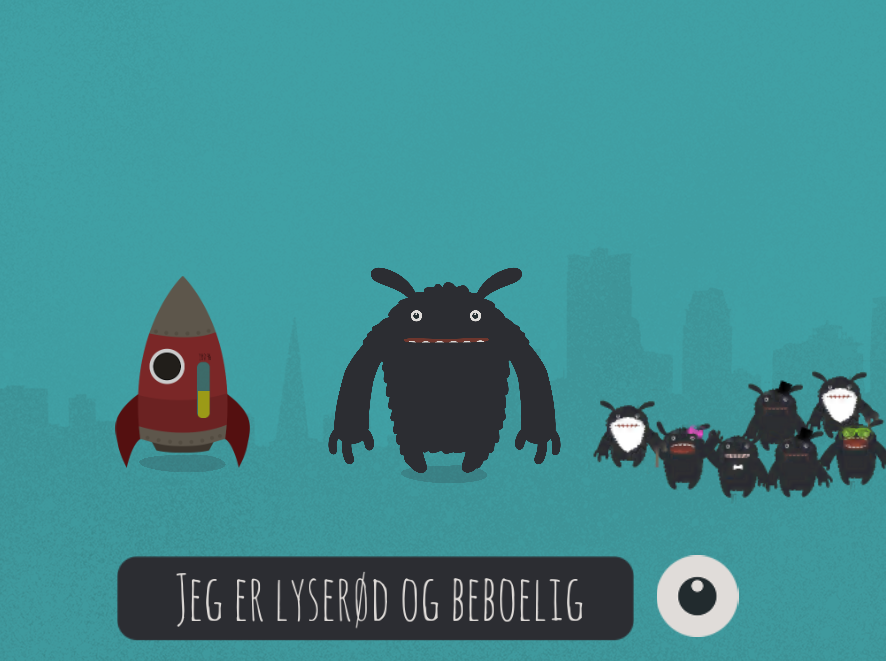
\includegraphics[scale=0.24]{Pics/riddles4.png}
\caption{Riddle-based navigation showing the monster character with points in the form of fuels and friends.}
\label{monster}
\end{figure}

Due to the importance of choice and interactive narratives in games, as earlier mentioned, players have the ability to choose whether the monster should look for fuel or friends, which will affect the outcome of the game. These choices are made at the street art paintings. Ideally, different routes should be used for different choices, however to minimize the amount of bias in the experiment, the illusion of choice is given, as the choice will only influence the outcome of the game, not the route to be taken. The choice is made through a dialogue with characters in the street art paintings, which starts as players augment the paintings at the POIs. To incorporate pedagogic elements, information about the painting itself is given through the dialogue, and after augmenting the painting, players unlock access to an info screen about the particular painting. This was included, in order to incorporate the element of saving information about places visited, mentioned previously by Gentes et al. \cite{GamingOnTheMove} and Peitzl et al. \cite{Insectopia}, giving the user a sense of progression and feedback. 

\begin{figure}[hbtp]
\centering
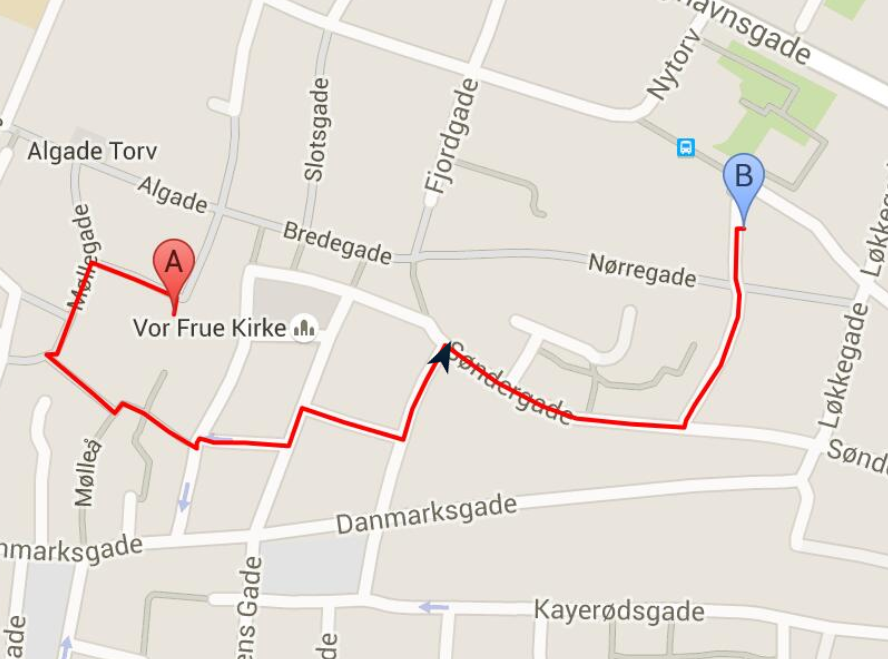
\includegraphics[scale=0.24]{Pics/MapNav.png}
\caption{Map-based navigation using map provided by Google Maps showing user's position}
\label{map}
\end{figure}

In the game activity between POIs, players use riddle solving while navigating, as earlier mentioned. When players start their first riddle, a tutorial introduces how the system works. To incorporate a feedback system, players are given points as they answer correctly on the control questions for the riddles. These points are dependant on the choice made at the previous POI, so for instance in the case that players have chosen to look for fuel, fuel points will be given to the players and vice versa (See Figure \ref{monster}). Whether the monster will get home or have any friends in the end of the game, will rely on this choice. We also implemented a 2D digital map into the game for the purpose of the experiment. The map had the primary objective of resembling maps used in other LBGs or a even simpler version, showing the user's position on a 2D digital map provided by Google Maps (See Figure \ref{map}). As seen in the LBG \textit{Team Exploration}, incorporating limitations in the game such as time, can cause the focus of the game to be more on the hunt itself and not the exploration that takes place in the physical space. For this reason, the limitations used in Lost on Earth are primarily found in the act of navigating itself, where using riddles to navigate is a cumbersome, but also enjoyable way of navigating, as it makes use of the physical space. 